%%%%%%%%%%%%%%%%%%%%%%%%%%%%%%%%%%%%%%%%%%%%%%%%%%%%%%%%%%%%%%%%%%%%%%
%%  dissertation.tex, to be compiled with latex2e.                   %
%%  16 April 2012                                                    %
%%%%%%%%%%%%%%%%%%%%%%%%%%%%%%%%%%%%%%%%%%%%%%%%%%%%%%%%%%%%%%%%%%%%%%
%%                                                                   %
%%  Writing a Doctoral Dissertation with LaTeX at                    %
%%           Georgia State University                                %
%%                                                                   %
%%  (Running this ``template'' will generate the documentation.)     %
%%                                                                   %
%%%%%%%%%%%%%%%%%%%%%%%%%%%%%%%%%%%%%%%%%%%%%%%%%%%%%%%%%%%%%%%%%%%%%%

%\documentclass[12pt,gsu,online,openright,doubleside]{gsudiss}
\documentclass[12pt,gsu,online,openany,singleside,hidelinks]{gsudiss}
\usepackage{natbib}
%\usepackage{subfigure}                % To format bibliographies.
%% \usepackage{aastex}
\setlength{\bibsep}{0pt}           % Necessary for bib entries to have
                                   % correct line spacing.
\usepackage{tocloft}
\usepackage[hidelinks]{hyperref}

\hypersetup{
    colorlinks=false,
    pdfborder={0 0 0},
}


\renewcommand{\cftfigfont}{Figure\ }
\renewcommand{\cfttabfont}{Table\ }
\renewcommand{\cftchapfont}{\bfseries}
\renewcommand{\cftsecfont}{\bfseries}
\renewcommand{\cftsubsecfont}{\bfseries\itshape}
\renewcommand{\cftsubsubsecfont}{\itshape}
\renewcommand{\cftparafont}{\mdseries}

\usepackage{lscape}
\usepackage{geometry}
\usepackage{array}
\usepackage{deluxetable}
%\usepackage{aastex_hack}
\usepackage{longtable,ltcaption}
\usepackage{float}
\usepackage[caption = false]{subfig}
% The ltcaption package supports \CaptionLabelFont & \CaptionTextFont
% introduced by the NTG document classes
\renewcommand\CaptionLabelFont{\normalsize}
\renewcommand\CaptionTextFont{\normalsize}
\usepackage{aas}                   % Some abbreviations for AAS references.
\citestyle{aa}                     % Astronomy & Astrophysics cite style.
\usepackage{eucal}                 % Euler fonts for equations.
\usepackage{verbatim}              % Allows quoting source with commands.
\usepackage{graphicx}              % For powerful manipulation of figures.
\usepackage{amsmath,amsthm,amsfonts,amsopn,amssymb} % Some nice math packages.
\usepackage{ctable}                % My preference table package.
\usepackage[overlay]{textpos}      % Put stuff anywhere, I mean anywhere ...
\usepackage{pstricks}              % Draw stuff especially on top figures etc...
\usepackage{afterpage}             % Useful for absolute placement of figures and tables.
\usepackage{longtable} % for 'longtable' environment
\usepackage{pdflscape} % for 'landscape' environment

%\input{figures}                    % My defined figures, see the file "figures.tex".
\newcommand\arcdeg{\mbox{\ensuremath{^\circ}}}%
\newcommand\arcmin{\mbox{\ensuremath{^\prime}}}%
\newcommand\arcsec{\mbox{\ensuremath{^{\prime\prime}}}}%
\newcommand{\point}{\mbox{\ensuremath{\!\!.}\thinspace}}
\newcommand{\minusone}{\ensuremath{^{-1}}}
\newcommand{\minustwo}{\ensuremath{^{-2}}}
\newcommand{\minusthree}{\ensuremath{^{-3}}}
\newcommand{\minusfive}{\ensuremath{^{-5}}}
\newcommand{\plusthree}{\ensuremath{^{3}}}
\newcommand{\plusfive}{\ensuremath{^{5}}}
\newcommand{\kms}{\mbox{\ km\,s\ensuremath{^{-1}}}}
\newcommand{\fig}{Figure~}
\newcommand{\figs}{Figures~}
\newcommand{\tab}{Table~}
\newcommand{\tabs}{Tables~}
\newcommand{\eqn}{Equation~}
\newcommand{\eqns}{Equations~}
\newcommand{\vracc}{\mbox{$\mathrm{v=kr}$}\xspace}
\newcommand{\vrdec}{\mbox{$\mathrm{v=v_{max}-k^{'}(r-r_t)}$}\xspace}
\newcommand{\vrootracc}{\mbox{$\mathrm{v=k_{1}\sqrt r}$}\xspace}
\newcommand{\vrootrdec}{\mbox{$\mathrm{v=v_{max}-k_{2}\sqrt{r-r_t}}$}\xspace}
\newcommand{\rlaw}{\mbox{$r\ $law}\xspace}
\newcommand{\rootrlaw}{\mbox{$\sqrt r\ $law}\xspace}
\newcommand{\resolvingpower}{\mbox{$\lambda/\Delta\lambda$}\xspace}
\newcommand{\OIII}{\mbox{[\acs{O3}]}\xspace}
\newcommand{\solarmass}{\mbox{\ M\ensuremath{_{\odot}}}}
\newcommand{\arcpt}{${{\lower3pt\hbox{$^{\prime\prime}$}}\atop{\raise4pt\hbox{.}}}$}
\newcommand{\msun}{$M_\odot$}

% ------------ Biblatex specific settings --------------- %

% Force sentence casing for article titles in bibliography
\DeclareFieldFormat{titlecase}{\MakeTitleCase{#1}}
\newrobustcmd{\MakeTitleCase}[1]{%
  \ifthenelse{\ifcurrentfield{booktitle}\OR\ifcurrentfield{booksubtitle}%
    \OR\ifcurrentfield{maintitle}\OR\ifcurrentfield{mainsubtitle}%
    \OR\ifcurrentfield{journaltitle}\OR\ifcurrentfield{journalsubtitle}%
    \OR\ifcurrentfield{issuetitle}\OR\ifcurrentfield{issuesubtitle}%
    \OR\ifentrytype{book}\OR\ifentrytype{mvbook}\OR\ifentrytype{bookinbook}%
    \OR\ifentrytype{booklet}\OR\ifentrytype{suppbook}%
    \OR\ifentrytype{collection}\OR\ifentrytype{mvcollection}%
    \OR\ifentrytype{suppcollection}\OR\ifentrytype{manual}%
    \OR\ifentrytype{periodical}\OR\ifentrytype{suppperiodical}%
    \OR\ifentrytype{proceedings}\OR\ifentrytype{mvproceedings}%
    \OR\ifentrytype{reference}\OR\ifentrytype{mvreference}%
    \OR\ifentrytype{report}\OR\ifentrytype{thesis}}
    {#1}
    {\MakeSentenceCase{#1}}}

% ------------------------------------------------------- %

% ------------ Glossary specific settings --------------- %

% Define our implementation for the listofabbreviations hook
\newcommand{\printabbreviations}{%
  \renewcommand{\glossarysection}[2][]{}
  \glsaddall
  \setlength{\LTleft}{0pt}
  \setlength{\LTright}{0pt}
  \vspace{-1.1\baselineskip}
  \renewcommand{\arraystretch}{1}
  \printnoidxglossary[type=acronym,style=mylong,toctitle=\loaname,nonumberlist]
}

\renewcommand{\glsnamefont}[1]{\textbf{#1}}
\loadglsentries{Frontmatter/abbreviations.tex}
\makenoidxglossaries

% Custom glossary formatting
\renewcommand{\glossentrydesc}[1]{%
  \glsentrylong{#1}%
  \ifglshasfield{user1}{#1}{%
    \space(``\glsuseri{#1}'')%
  }{}%
}

% Commands for alternate glossary terms
\newcommand{\altgls}[1]{%
  \ifglshasfield{user1}{#1}{%
    \glsuseri{#1}%
  }{%
    \gls{#1}%
  }%
}

\newcommand{\altglspl}[1]{%
  \ifglshasfield{user1}{#1}{%
    \glsuseri{#1}s%
  }{%
    \glspl{#1}%
  }%
}

% ------------------------------------------------------- %

% ------------------ SI unit commands ------------------- %

% Declare some new SI units
\DeclareSIUnit{\fps}{fps}      % frames per second
\DeclareSIUnit{\cps}{cps}      % cycles per second
\DeclareSIUnit{\cpd}{cpd}      % cycles per degree
\DeclareSIUnit{\rpm}{rpm}      % rotations per minute
\DeclareSIUnit{\mM}{mM}        % millimolar

% ------------------------------------------------------- %

% ------------------- Appendix setup -------------------- %

% Prefixes Appendix X figures, tables, and equations with X

\newcommand{\setupappendix}[1]{%
  \renewcommand{\thefigure}{#1\arabic{figure}}%
  \renewcommand{\thetable}{#1\arabic{table}}%
  \renewcommand{\theequation}{#1\arabic{equation}}%
  \setcounter{figure}{0}%
  \setcounter{table}{0}%
  \setcounter{equation}{0}%
}

% ------------------------------------------------------- %

               % User defined commands go in this
                                   % file called "usercommands.tex".
                                   % Of course you can rename it.
\usepackage{float}
\floatstyle{boxed}
\newfloat{code}{h}{ext}
\floatname{code}{Code}


\usepackage{fancyvrb}
\DefineVerbatimEnvironment{code}{Verbatim}{fontsize=\small}
\DefineVerbatimEnvironment{example}{Verbatim}{fontsize=\small}




\usepackage{atbeginend}            % Modify space before and after
                                   % equations. These are my preferences.
\AfterBegin{equation}{\addtolength{\abovedisplayskip}{-0.5\baselineskip}}
\BeforeEnd{equation}{\addtolength{\belowdisplayskip}{-0.5\baselineskip}}
\AfterBegin{equation*}{\addtolength{\abovedisplayskip}{-0.5\baselineskip}}
\BeforeEnd{equation*}{\addtolength{\belowdisplayskip}{-0.5\baselineskip}}

\renewcommand{\topfraction}{0.85}        % These modify figure placement on
\renewcommand{\bottomfraction}{0.85}     % the page and various other space
\renewcommand{\textfraction}{0.10}       % requirements for figures.
\renewcommand{\floatpagefraction}{0.80}  % These 5 lines are not
\renewcommand{\arraystretch}{0.5}        % necessary but I think its better
                                         % than latex default.

\setlength{\tabcolsep}{3pt}        % shrink column spacing so your tables 
                                   % can be wider (yay Todd Tables)
%\setlength{\LTcapwidth}{\textwidth}% so your rotated, normal-sized
                                   % longtable titles won't wrap oddly.



\clubpenalty=1000                  % Make Latex try hard to fix
\widowpenalty=1000                 % "stray lines" in paragraphs,
                                   % i.e. paragraph that begin at the
                                   % last line of a page, or end with
                                   % the last line on the following
                                   % page. This looks silly.
\raggedbottom

\settocname{TABLE OF CONTENTS}              % Set the "Table of Contents"
                                   % name. This is the default. You
                                   % can use "Table of Contents" for example.

\setlofname{LIST OF FIGURES}               % Change the name from 'List of
                                   % Figures'. Use whatever you wish.

\setlotname{LIST OF TABLES}                % Change the name from 'List of
                                   % Tables'. Use whatever suit your
                                   % fancy.

\settocbibname{REFERENCES}         % Change the name from
                                   % 'Bibliography'. Change it back if
                                   % you feel like it.

\setloaname{LIST OF ABBREVIATIONS}
                                   % I Changed the name from 'List of
                                   % Abbreviations'. Use any name that
                                   % makes sense here. If you don't
                                   % have an "abbreviations.tex" file,
                                   % this command will do nothing.

\setfigname{Figure\ }               % Set the caption labels for figures.

\settabname{Table\ }                % Set the caption labels for tables.

\setcapfont{pnc}                   % Set the caption font for
                                   % both tables and figures.

\chapternumsize{\normalsize}            % You can use any standard latex sizes here.
\chapterheadsize{\normalsize}           % You can use any standard latex sizes here.
\chaptertitlesize{\normalsize}           % You can use any standard latex sizes here.
                                   % These defaults look good to me.

\beforechapterheadname{CHAPTER}         % Optional text to put in front of
                                   % the chapter number.
\afterchapterheadname{}          % Optional text to put after the
                                   % chapter number. The default
                                   % looks like this: --1--. Of course
                                   % you can change this to any
                                   % format, for e.g. $\sim$

\chapterheadpos{center}            % You can use 'right', 'left',
                                   % 'center'.

\chaptertitlepos{center}           % You can use 'right', 'left',
                                   % 'center'

\chapterheadverticalspace{-1em}     % The space between the Chapter head
                                   % and the top of page. This distance
                                   % is not absolute, but relative to
                                   % the parameters set by the
                                   % geometry package. Play around
                                   % with this number to suit your needs.

\chapterbetweentitlespace{-1.em}   % The space between the chapter head
                                   % and the title head.

\titleheadverticalspace{2em}       % The space between the title head
                                   % and the text.

\sectiontitlesize{\normalsize}          % This is obvious.
\sectiontitlepos{left}             % Obvious.

\sectiontitleverticalspace{1em}    % The space between the section head
                                   % and the text.

\subsectiontitlesize{\normalsize}       % Obvious.
\subsectiontitlepos{left}          % Obvious.

\subsectiontitleverticalspace{0.5em} % You get the idea...

\subsubsectiontitlesize{\normalsize}
\subsubsectiontitlepos{left}

\subsubsectiontitleverticalspace{0.5em}

\sepabbrev{7em}                    % The space between the abbreviation
                                   % lists, that is, if you have
                                   % one. Has to be >= 5em.

\prettify{pnc}

\printdraft{\textcolor{gray}\small DRAFT}    % In order to use this
                                   % command, you have to enable "drafts"
                                   % in the option of the gsudiss
                                   % class, otherwise it does
                                   % nothing. This prints the word
                                   % "DRAFT" in gray color in the header of your
                                   % dissertation. You can go wild
                                   % here if you want. Just make sure
                                   % you disable the draft option
                                   % before final printing.

\author(First and Last Name)              % Name required.

\title(Your Title in Title Caps)    % Title of dissertation Required.

\titlesize(11)(11)                               % This is for changing
                                             % the default font size
                                             % for your title. The
                                             % first argument is the
                                             % font size, the second
                                             % is the line spacing for
                                             % long tiles that wrap to
                                             % more than one line.
                                             % Default is equivalent
                                             % to the \LARGE command,
                                             % which is roughly (22)(22).

% \committee: The first parenthesis must contain your supervisor name.
%         You can have two supervisors, in which case, the
%         second supervisor goes into the square brackets, next to the
%         first. If you have one like me, then leave the second entry blank, like below. The
%         rest of the parentheses contains the rest of your committee members. You
%         can have up to six entries, NOT including your supervisor(s). My
%         school requires five or four. I have five (5) members
%         below. Note that there is no need to put the "Dr." title in front of any of the names.
% Adjust margins to 1.0in on all sides

\committee(Committee Chair)[]
          (Committee Member)
          (Committee Member)
          (Committee Member)
          (Committee Member)

\department(Department of Physics and Astronomy)
                                   % Your Department name.
                                   % Other departments you can
                                   % use include
                                   % \department(School of Arts \& Design)
                                   % or \department(School of Music), etc...

\departmenttitle(Chair)            % For Arts and Music school
                                   % students use
                                   % \departmenttitle{Director}

\graduationyear(YEAR)              % Defaults to the same year
                                   % you are writing this
                                   % Dissertation. Do
                                   % \graduationyear(200x) if
                                   % you ever need to change it.

\graduationmonth(Month)           % This is the date of the
                                   % official graduation ceremony.
                                   % Do \graduationmonth{January}
                                   % for example. Defaults to "August"
\newcommand\omicron{o}

%%%%%%%%%%%%%%%%%%%%%%%%%%%%%%%%%%%%%%%%%%%%%%%%%%%%%%%%%%%%%%%%%%%%%%
%               The dissertation starts here.                        %
%%%%%%%%%%%%%%%%%%%%%%%%%%%%%%%%%%%%%%%%%%%%%%%%%%%%%%%%%%%%%%%%%%%%%%

\begin{document}
\pagestyle{empty}
\begin{center}
%\vspace*{.1in}
Sample Title in Title Caps

\vspace{.9in}
by\\
\vspace{.9in}
First and Last Name\\
\vspace{.9in}
Under the Direction of Committee Chair's First and Last Name, Ph.D. \\
\vspace{2in}

A Dissertation/Thesis Submitted in Partial Fulfillment of the Requirements for the Degree of\\  % Choose either thesis or dissertation and delete the other.
\vspace{.2in}
Doctor of Philosophy/Master of Science \\
\vspace{.2in}
in the College of Arts and Sciences \\
\vspace{.2in}
Georgia State University \\
\vspace{.2in}
Year
\pagebreak 



ABSTRACT\\
\bigskip
\end{center}


Your abstract must be in place at the time of initial submission. In MS theses, the abstract cannot exceed 150-words. In doctoral dissertations, the abstract cannot exceed 350-words. 


\begin{singlespace}
\vspace{0.5in}
\noindent INDEX WORDS:
\hspace{0.2in}
\parbox[t]{4.5in}{
Sample index words, Sample, Sample, Sample}
\end{singlespace}             % See the TitleAbstract.tex file
%%%%%%%%%%%%%%%%%%%% The front matter of your document %%%%%%%%%%%%%%%%%%%%


\frontmatter

\certifypage                 % Produces the certify page, if this option is
                             % set in the class file.



\copyrightpage               % Produces the copyright page.
\clearpage
\approvalpage                % Produces the approval page.
\clearpage
\dedicationpage              % The dedication page is optional.
\clearpage                             % This command does nothing if you don't
                             % have a `dedication.tex' file, otherwise
                             % the file is included in the frontmatter.

\acknowledgmentpage          % The acknowledge page is optional.
\clearpage                             % This command does nothing if you don't
                             % have an `acknowledgment.tex' file, otherwise
                             % the file is included in the frontmatter.

\tableofcontents             % Table of Contents will be automatically
\clearpage                             % generated and placed here.

\listoftables                % List of Tables will be automatically
\clearpage                             % generated if you had made proper table captions.

\listoffigures               % List of Figures will be automatically
\clearpage                             % generated if you had made proper figure captions.

\listofabbreviations         % List of Abbreviations will be
\clearpage                             % automatically generated if you had made any,
                             % following the style of the "Acronym"
                             % package. See my "abbreviation.tex" file
                             % for example usage. If you don't have
                             % this file, the command does nothing.
              % See the frontmatter.tex file

\mainmatter                        % Main chapters starts here
\chapter{CHAPTER 1 TITLE}

\section{The First Section of the First Chapter}
	You should probably introduce some stuff here
    
    You should look at the gsudiss.cls file first when you want to change things in how the document is laid out (also, the `Copyright by Your Name' bit is hard-coded there, so you'll have to change that).
\chapter{CHAPTER 2 TITLE}

Hooray for Chapter 2!!!

Sample Figures and Tables below.

And as an example of citing things, I'm going to cite a brilliant paper - \citep{jones_2016}. See bibliography.bib for doing references.

\begin{figure*}
	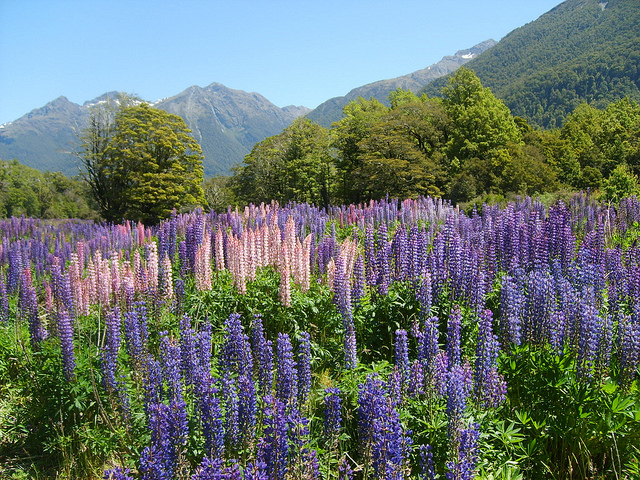
\includegraphics[height =5in]{./Plots/nature.jpg}
	\caption{An individual figure!}
\end{figure*}
        
\begin{figure*}[h]
	\subfloat[\label{fig:HD8538_ellplot}]{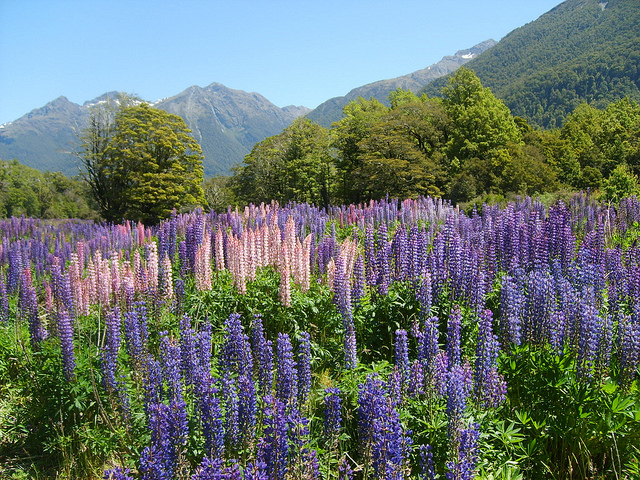
\includegraphics[height =2.5in]{./Plots/nature.jpg}} 
	\subfloat[\label{fig:HD8538_phot}]{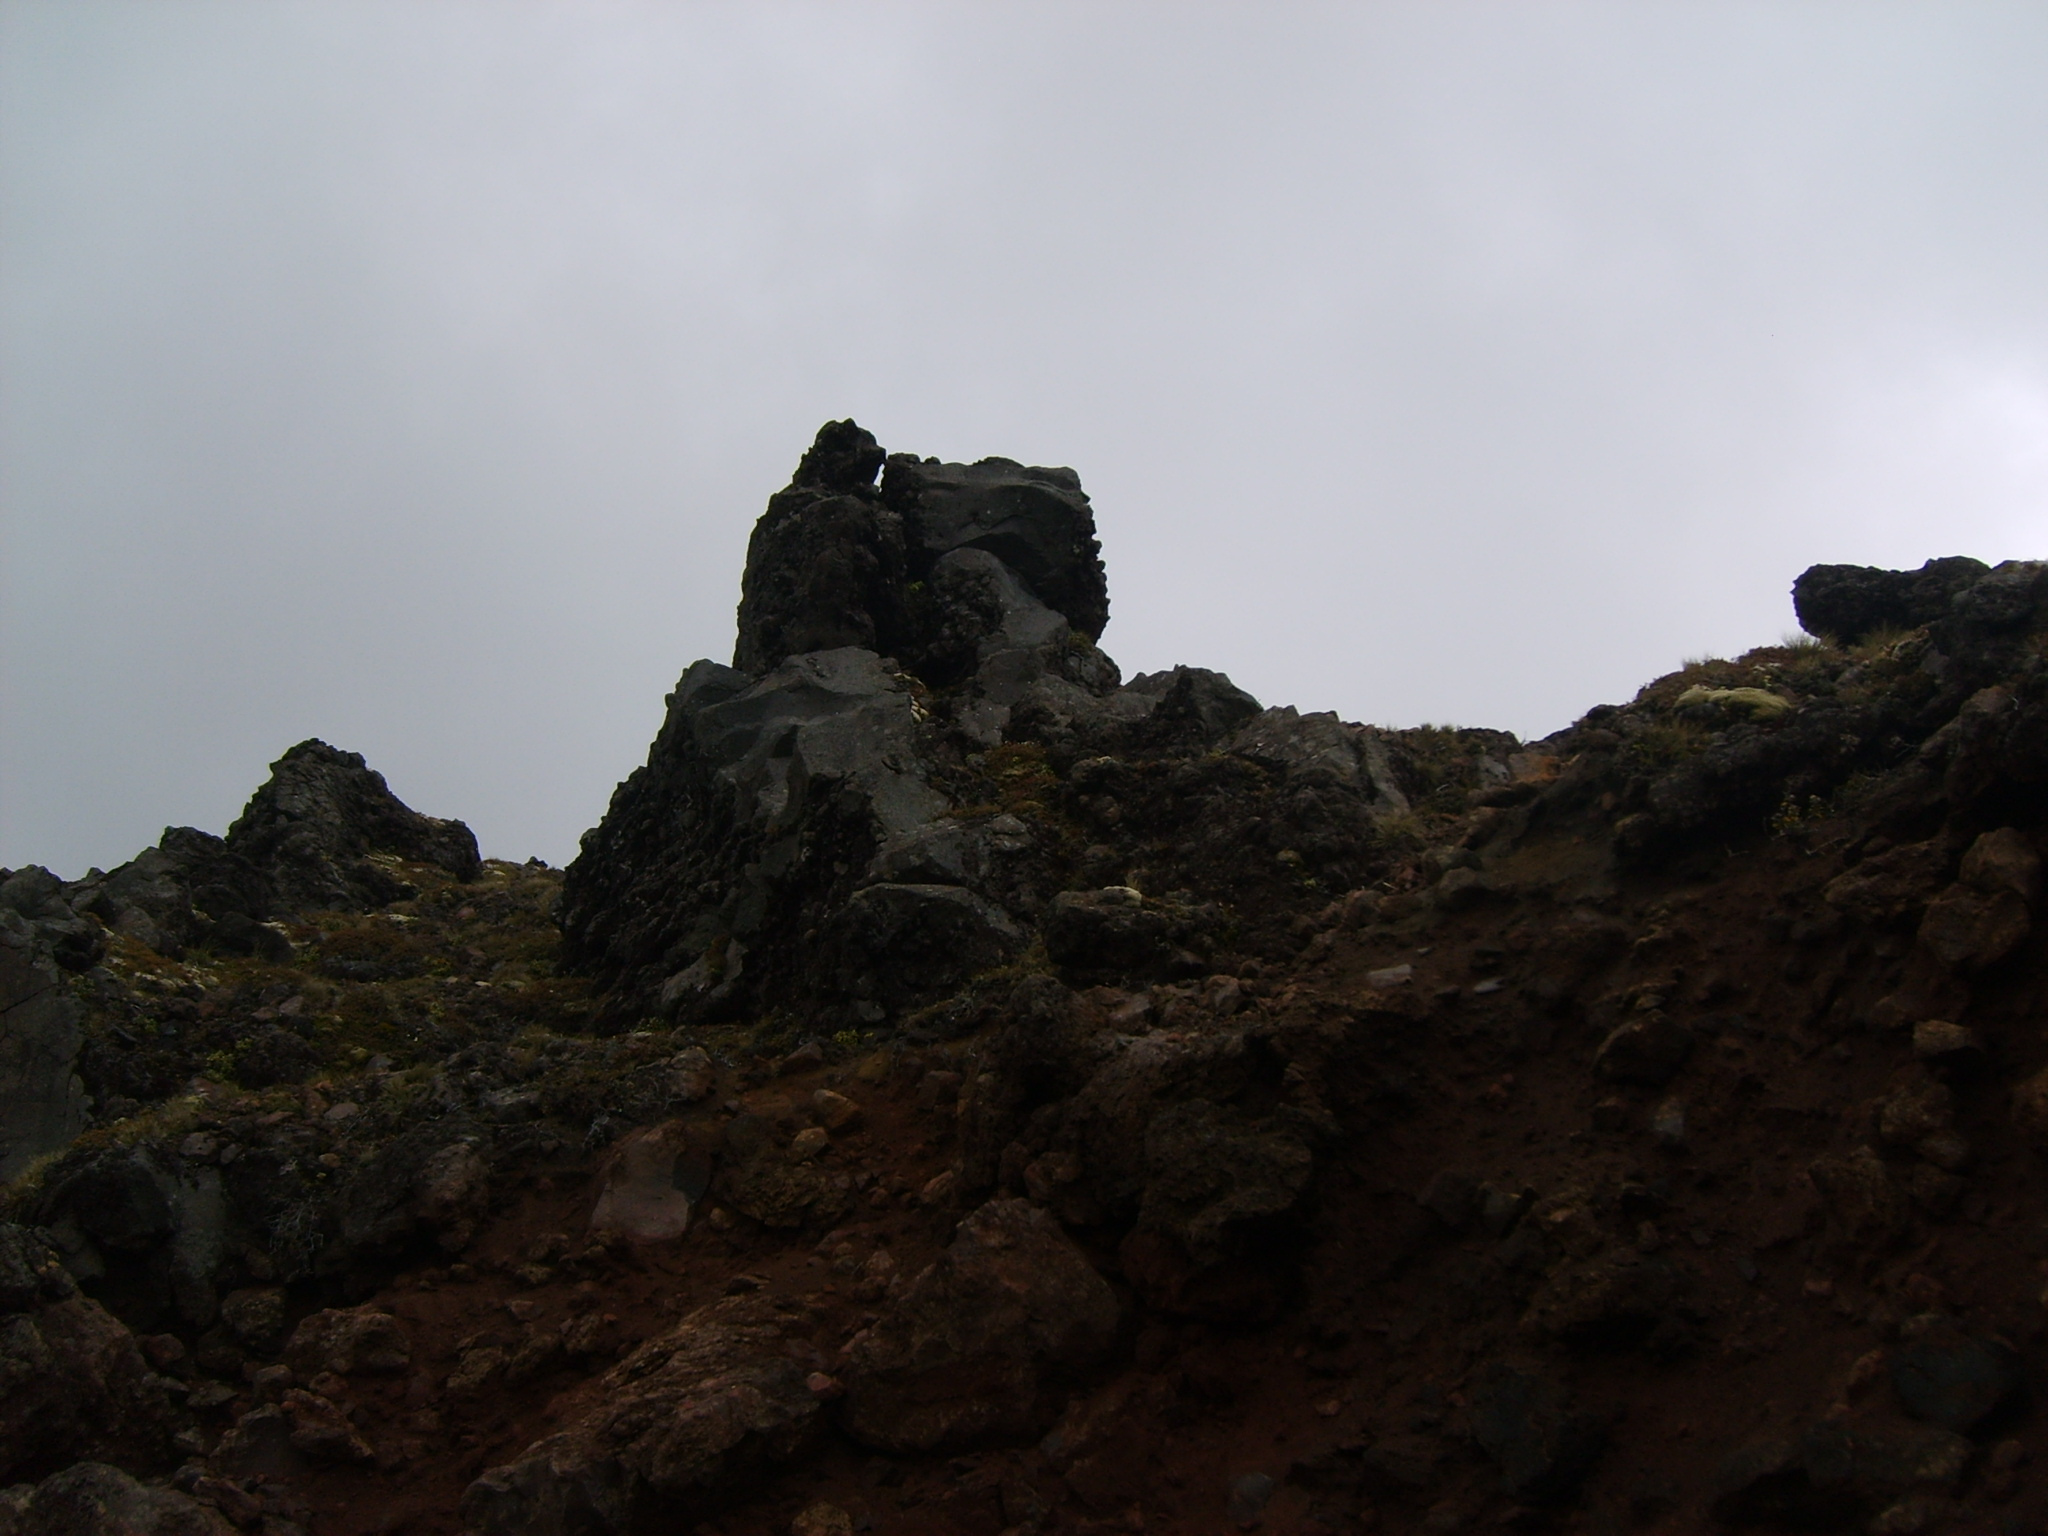
\includegraphics[height =2.5in]{./Plots/rocks.jpg}} \\
	\subfloat[\label{fig:HD8538_vis}]{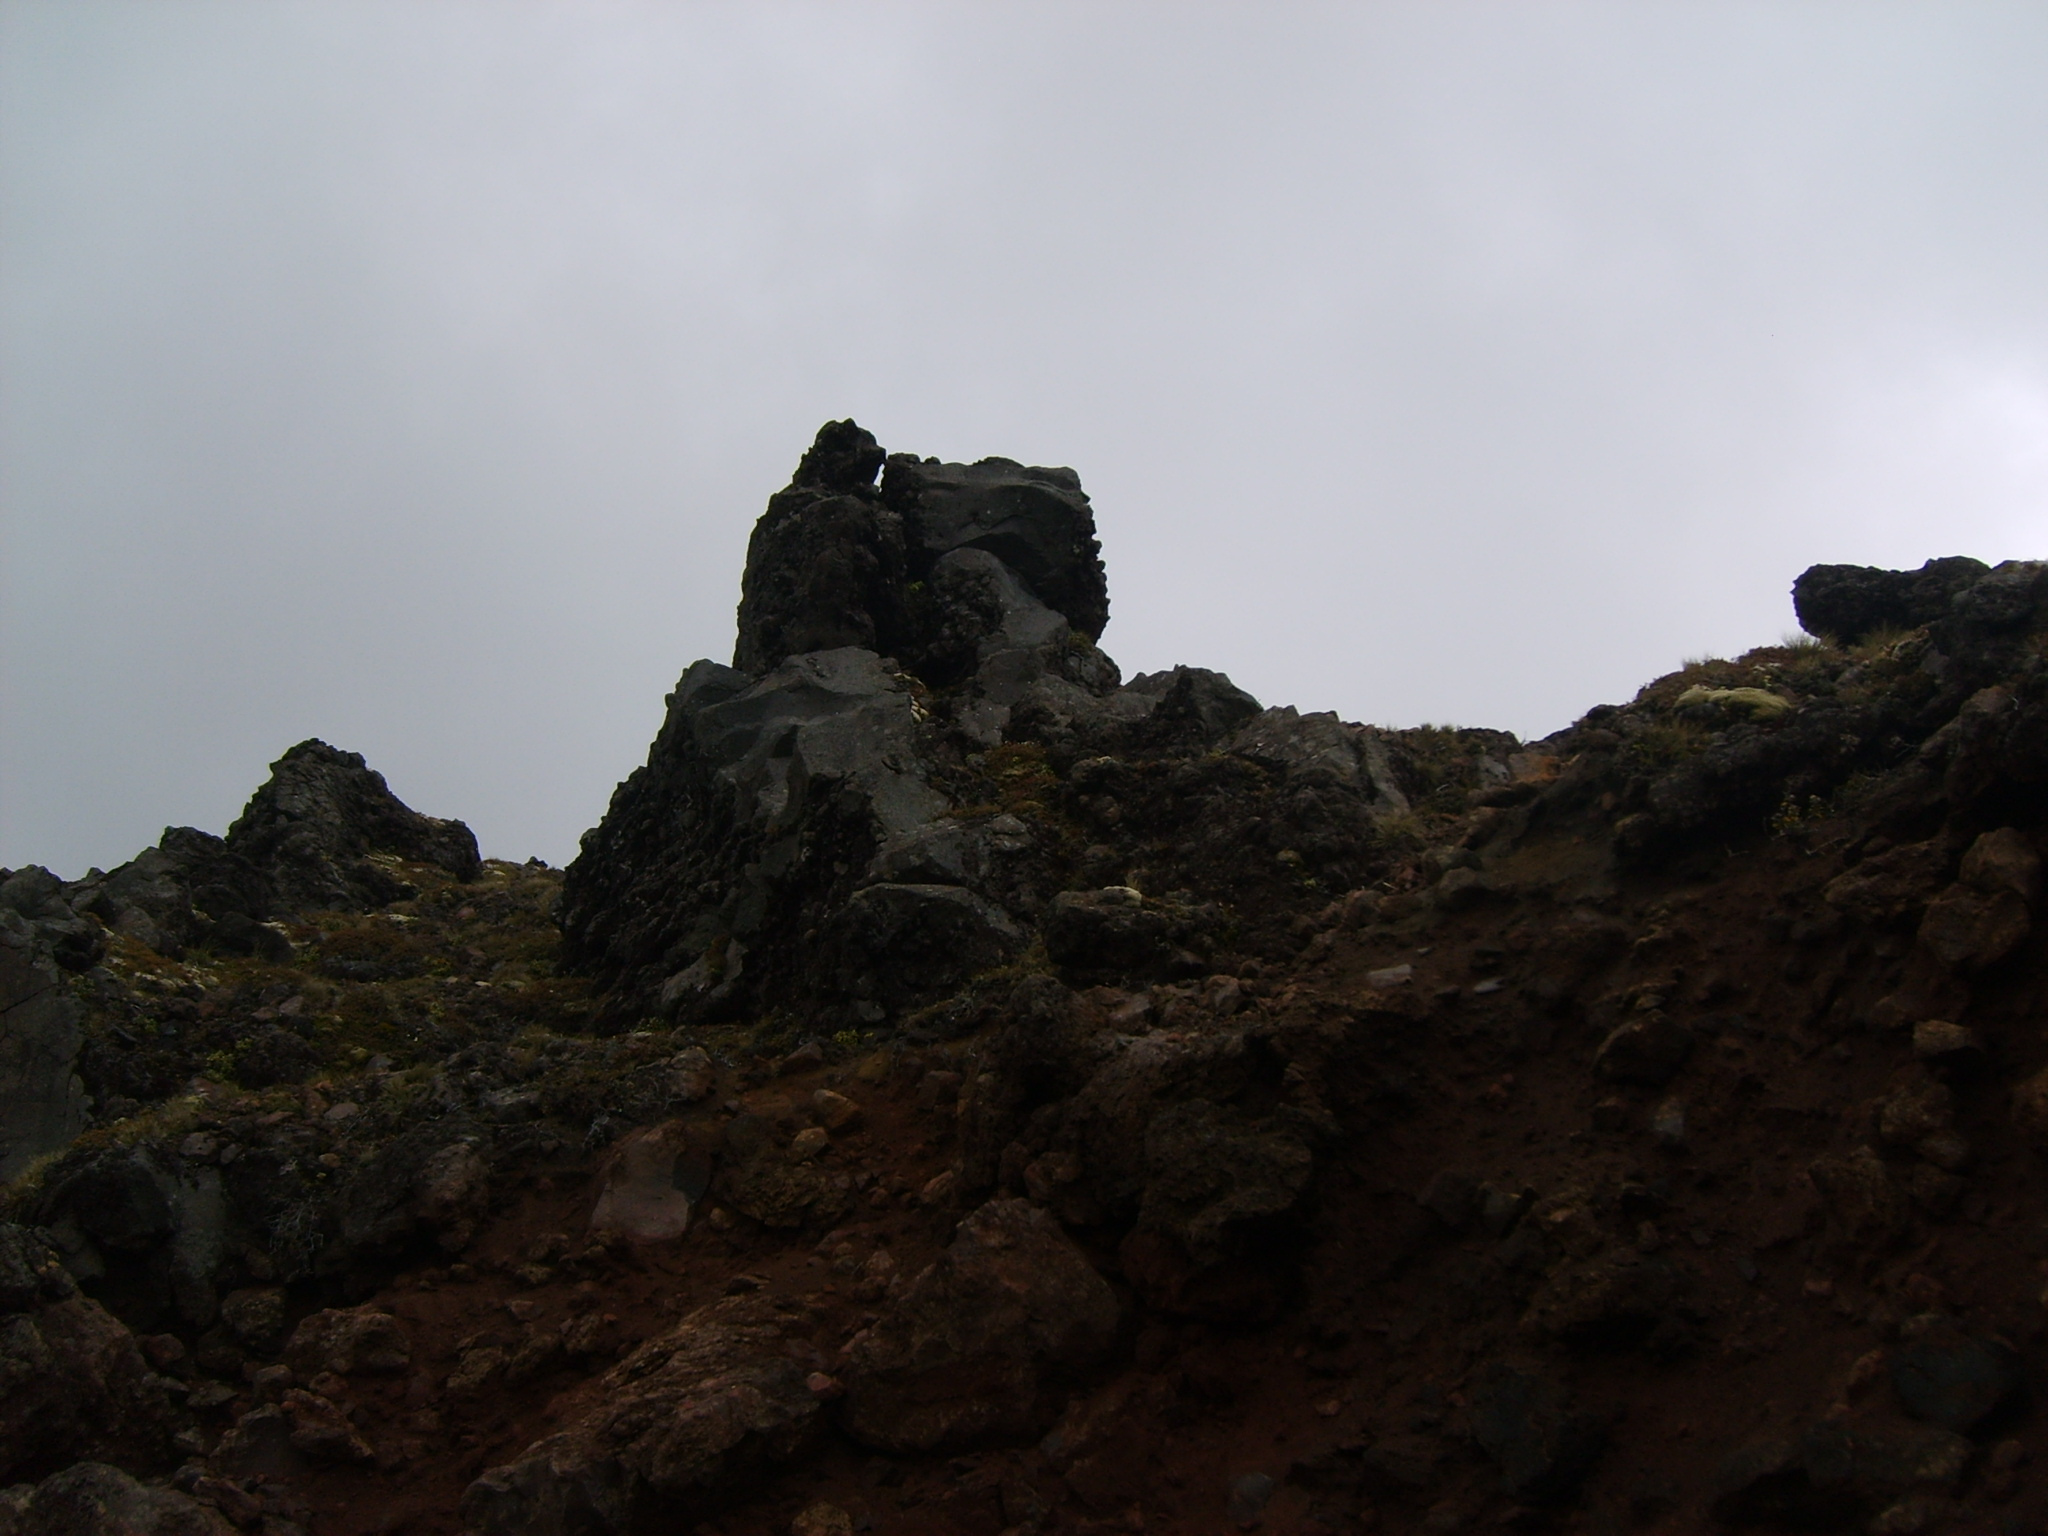
\includegraphics[height =2.5in]{./Plots/rocks.jpg}}
	\subfloat[\label{fig:HD8538_HRD}]{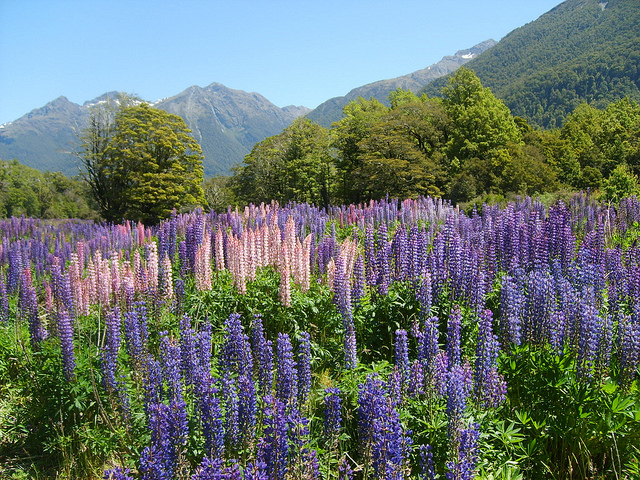
\includegraphics[height =2.5in]{./Plots/nature.jpg}}
	\caption{Multiple figures!}
\end{figure*}



\begin{landscape}
\begin{longtable}{cccccccccccccc}
\label{tab:disk}\\
\caption{Insert Table Caption here}\\
\hline\endhead  % header material
\hline\endfoot  % footer material
\hline
Blah & Blah & Blah \\
\hline
Stuff & Things & etc. \\
\nodata & \nodata & \nodata \\
\end{longtable}
\end{landscape}


\appendix
\section*{Appendices}
\addcontentsline{toc}{section}{Appendices}
\renewcommand{\thesubsection}{\Alph{subsection}}

\documentclass[../../main.tex]{subfiles}  % Two levels up to main.tex
\begin{document}

\section{Something}
This is the appendix!

\end{document}
\section{Something Else}
Another appendix!

%%%%%%%%%%%%%%%%%%%% The backmatter goes in this file %%%%%%%%%%%%%%%%%%%%%

% The bibliography starts here.

% original CAS template used the below for 'natbib' -- uncomment the below two \bibliography{} commands and comment out \setlength and \printbibliography for natbib
% \bibliographystyle{apj}             % Please learn to use the
                                    % formatting of Latex's Bibtex. It
                                    % will make your life easier.

% \bibliography{bibliography}

%\bibliography{apj-jour,dissref}       % "paper.bib" contains all my
                                    % references. "apj-jour.bib"
                                    % contains abbreviations of
                                    % journals.

% added to switch to biblatex
\setlength\bibitemsep{0pt}   % if using biblatex
\printbibliography


\clearpage
% If you have only one appendix chapter, use the command
% \begin{appendix}...\end{appendix} instead.
% This takes care of the requirement (of the Graduate Office) for one
% appendix chapter to be labeled as 'Appendix', not 'Appendix A'.

\beforechapterheadname{APPENDIX}         % Optional text to put in front of
                                   % the chapter number.
\afterchapterheadname{}          % Optional text to put after the

\addcontentsline{toc}{chapter}{APPENDIX}

%\begin{appendix}
%  \input{appendixI}                     % Your appendices go here.
%  %%
%% This is file `appendix.sty',
%% generated with the docstrip utility.
%%
%% The original source files were:
%%
%% appendix.dtx  (with options: `usc')
%%
%% -----------------------------------------------------------------
%%   Author: Peter Wilson (CUA) now at peter.r.wilson@boeing.com until June 2004
%%                              (or at: pandgwilson at earthlink dot net)
%%   Copyright 1998 --- 2004 Peter R. Wilson
%%
%%   This work may be distributed and/or modified under the
%%   conditions of the LaTeX Project Public License, either
%%   version 1.3 of this license or (at your option) any
%%   later version.
%%   The latest version of the license is in
%%      http://www.latex-project.org/lppl.txt
%%   and version 1.3 or later is part of all distributions of
%%   LaTeX version 2003/06/01 or later.
%%
%%   This work has the LPPL maintenance status "author-maintained".
%%
%%   This work consists of the files listed in the README file.
%% -----------------------------------------------------------------
%%
\NeedsTeXFormat{LaTeX2e}
\ProvidesPackage{appendix}[2002/08/06 v1.2 extra appendix facilities]

\newif\if@chapter@pp\@chapter@ppfalse
\newif\if@knownclass@pp\@knownclass@ppfalse
\@ifundefined{chapter}{%
  \@ifundefined{section}{}{\@knownclass@pptrue}}{%
  \@chapter@pptrue\@knownclass@pptrue}
\providecommand{\phantomsection}{}
\newcounter{@pps}
  \renewcommand{\the@pps}{\alph{@pps}}
\newif\if@pphyper
  \@pphyperfalse
\AtBeginDocument{%
  \@ifpackageloaded{hyperref}{\@pphypertrue}{}}

\newif\if@dotoc@pp\@dotoc@ppfalse
\newif\if@dotitle@pp\@dotitle@ppfalse
\newif\if@dotitletoc@pp\@dotitletoc@ppfalse
\newif\if@dohead@pp\@dohead@ppfalse
\newif\if@dopage@pp\@dopage@ppfalse
\DeclareOption{toc}{\@dotoc@pptrue}
\DeclareOption{title}{\@dotitle@pptrue}
\DeclareOption{titletoc}{\@dotitletoc@pptrue}
\DeclareOption{header}{\@dohead@pptrue}
\DeclareOption{page}{\@dopage@pptrue}
\ProcessOptions\relax
\newcommand{\@ppendinput}{}
\if@knownclass@pp\else
  \PackageWarningNoLine{appendix}%
    {There is no \protect\chapter\space or \protect\section\space command.\MessageBreak
     The appendix package will not be used}
  \renewcommand{\@ppendinput}{\endinput}
\fi
\@ppendinput

\newcommand{\appendixtocon}{\@dotoc@pptrue}
\newcommand{\appendixtocoff}{\@dotoc@ppfalse}
\newcommand{\appendixpageon}{\@dopage@pptrue}
\newcommand{\appendixpageoff}{\@dopage@ppfalse}
\newcommand{\appendixtitleon}{\@dotitle@pptrue}
\newcommand{\appendixtitleoff}{\@dotitle@ppfalse}
\newcommand{\appendixtitletocon}{\@dotitletoc@pptrue}
\newcommand{\appendixtitletocoff}{\@dotitletoc@ppfalse}
\newcommand{\appendixheaderon}{\@dohead@pptrue}
\newcommand{\appendixheaderoff}{\@dohead@ppfalse}
\newcounter{@ppsavesec}
\newcounter{@ppsaveapp}
\setcounter{@ppsaveapp}{0}
\newcommand{\@ppsavesec}{%
  \if@chapter@pp \setcounter{@ppsavesec}{\value{chapter}} \else
                 \setcounter{@ppsavesec}{\value{section}} \fi}
\newcommand{\@pprestoresec}{%
  \if@chapter@pp \setcounter{chapter}{\value{@ppsavesec}} \else
                 \setcounter{section}{\value{@ppsavesec}} \fi}
\newcommand{\@ppsaveapp}{%
  \if@chapter@pp \setcounter{@ppsaveapp}{\value{chapter}} \else
                 \setcounter{@ppsaveapp}{\value{section}} \fi}
\newcommand{\restoreapp}{%
  \if@chapter@pp \setcounter{chapter}{\value{@ppsaveapp}} \else
                 \setcounter{section}{\value{@ppsaveapp}} \fi}
\providecommand{\appendixname}{APPENDIX}
\newcommand{\appendixtocname}{APPENDICES}
\newcommand{\appendixpagename}{APPENDICES}
\newcommand{\appendixpage}{%
%  \if@chapter@pp \@chap@pppage \else \@sec@pppage \fi
  \if@chapter@pp \else \@sec@pppage \fi
}
\newcommand{\clear@ppage}{%
  \if@openright\cleardoublepage\else\clearpage\fi}

\newcommand{\@chap@pppage}{%
%  \clear@ppage
%  \thispagestyle{plain}%
  \if@twocolumn\onecolumn\@tempswatrue\else\@tempswafalse\fi
%  \null\vfil
%  \markboth{}{}%
  {\centering
%   \interlinepenalty \@M
   \normalfont
   \normalsize \bfseries \appendixpagename\par}%
  \if@dotoc@pp
    \addappheadtotoc
  \fi
  \vfil%\newpage
  \if@twoside
    \if@openright
%      \null
%      \thispagestyle{empty}%
      %\newpage
    \fi
  \fi
  \if@tempswa
    \twocolumn
  \fi
}

\newcommand{\@sec@pppage}{%
  \par
  \addvspace{4ex}%
  \@afterindentfalse
  {\parindent \z@ \raggedright
   \interlinepenalty \@M
   \normalfont
   \normalsize \bfseries \appendixpagename%
   \markboth{}{}\par}%
  \if@dotoc@pp
    \addappheadtotoc
  \fi
  \nobreak
  \vskip 3ex
  \@afterheading
}

\newif\if@pptocpage
  \@pptocpagetrue
\newcommand{\noappendicestocpagenum}{\@pptocpagefalse}
\newcommand{\appendicestocpagenum}{\@pptocpagetrue}
\newcommand{\addappheadtotoc}{%
  \phantomsection
  \if@chapter@pp
    \if@pptocpage
      \addcontentsline{toc}{chapter}{\appendixtocname}%
    \else
      \if@pphyper
        \addtocontents{toc}%
          {\protect\contentsline{chapter}{\appendixtocname}{}{\@currentHref}}%
      \else
        \addtocontents{toc}%
          {\protect\contentsline{chapter}{\appendixtocname}{}}%
      \fi
    \fi
  \else
    \if@pptocpage
      \addcontentsline{toc}{section}{\appendixtocname}%
    \else
      \if@pphyper
        \addtocontents{toc}%
          {\protect\contentsline{section}{\appendixtocname}{}{\@currentHref}}%
      \else
        \addtocontents{toc}%
          {\protect\contentsline{section}{\appendixtocname}{}}%
      \fi
    \fi
  \fi
}

\providecommand{\theH@pps}{\alph{@pps}}

\newcommand{\@resets@pp}{\par
  \@ppsavesec
  \stepcounter{@pps}
  \setcounter{section}{0}%
  \if@chapter@pp
    \setcounter{chapter}{0}%
    \renewcommand\@chapapp{\appendixname}%
     \ifthenelse{\equal{\thechapter}{}}{\renewcommand\thesection{\@Alph\c@section}}{\renewcommand\thechapter{\@Alph\c@chapter}}
  \else
    \setcounter{subsection}{0}%
    \renewcommand\thesection{\@Alph\c@section}%
  \fi
  \if@pphyper
    \if@chapter@pp
      \renewcommand{\theHchapter}{\theH@pps.\Alph{chapter}}%
    \else
      \renewcommand{\theHsection}{\theH@pps.\Alph{section}}%
    \fi
    \def\Hy@chapapp{\appendixname}%
  \fi
  \restoreapp
}

\newenvironment{appendices}{%
  \@resets@pp
  \if@dotoc@pp
    \if@dopage@pp              % both page and toc
      \if@chapter@pp           % chapters
%        \clear@ppage
      \fi
      \appendixpage
    \else                      % toc only
       \if@chapter@pp          % chapters
%         \clear@ppage
       \fi
      \addappheadtotoc
    \fi
  \else
    \if@dopage@pp              % page only
      \appendixpage
    \fi
  \fi
  \if@chapter@pp
    \if@dotitletoc@pp \@redotocentry@pp{chapter} \fi
  \else
    \if@dotitletoc@pp \@redotocentry@pp{section} \fi
    \if@dohead@pp
      \def\sectionmark##1{%
        \if@twoside
          \markboth{\@formatsecmark@pp{##1}}{}
        \else
          \markright{\@formatsecmark@pp{##1}}{}
        \fi}
    \fi
    \if@dotitle@pp
      \def\sectionname{\appendixname}
      \def\@seccntformat##1{\@ifundefined{##1name}{}{\csname ##1name\endcsname\ }%
        \csname the##1\endcsname\quad}
    \fi
  \fi}{%
  \@ppsaveapp\@pprestoresec}

\newcommand{\setthesection}{\thechapter.\Alph{section}}
\newcommand{\setthesubsection}{\thesection.\Alph{subsection}}

\newcommand{\@resets@ppsub}{\par
  \stepcounter{@pps}
  \if@chapter@pp
    \setcounter{section}{0}
    \renewcommand{\thesection}{\setthesection}
  \else
    \setcounter{subsection}{0}
    \renewcommand{\thesubsection}{\setthesubsection}
  \fi
  \if@pphyper
    \if@chapter@pp
      \renewcommand{\theHsection}{\theH@pps.\setthesection}%
    \else
      \renewcommand{\theHsubsection}{\theH@pps.\setthesubsection}%
    \fi
    \def\Hy@chapapp{\appendixname}%
  \fi
}

\newenvironment{subappendices}{%
  \@resets@ppsub
  \if@chapter@pp
    \if@dotitletoc@pp \@redotocentry@pp{section} \fi
    \if@dotitle@pp
      \def\sectionname{\appendixname}
      \def\@seccntformat##1{\@ifundefined{##1name}{}{\csname ##1name\endcsname\ }%
        \csname the##1\endcsname\quad}
    \fi
  \else
    \if@dotitletoc@pp \@redotocentry@pp{subsection} \fi
    \if@dotitle@pp
      \def\subsectionname{\appendixname}
      \def\@seccntformat##1{\@ifundefined{##1name}{}{\csname ##1name\endcsname\ }%
        \csname the##1\endcsname\quad}
    \fi
  \fi}{}

\newcommand{\@formatsecmark@pp}[1]{%
  \MakeUppercase{\appendixname\space
    \ifnum \c@secnumdepth >\z@
      \thesection\quad
    \fi
    #1}}
\newcommand{\@redotocentry@pp}[1]{%
  \let\oldacl@pp=\addcontentsline
  \def\addcontentsline##1##2##3{%
    \def\@pptempa{##1}\def\@pptempb{toc}%
    \ifx\@pptempa\@pptempb
      \def\@pptempa{##2}\def\@pptempb{#1}%
      \ifx\@pptempa\@pptempb
\oldacl@pp{##1}{##2}{\appendixname\space ##3}%
      \else
        \oldacl@pp{##1}{##2}{##3}%
      \fi
    \else
      \oldacl@pp{##1}{##2}{##3}%
    \fi}
}

\endinput
%%
%% End of file `appendix.sty'.
                     %named "appendix.tex"
%\end{appendix}
               % See the backmatter.tex file


%%%%%%%%%%%%%%%%%%%%%%%%%%%%%%%%%%%%%%%%%%%%%%%%%%%%%%%%%%%%%%%%%%%%%%
%               The dissertation ends here.                          %
%%%%%%%%%%%%%%%%%%%%%%%%%%%%%%%%%%%%%%%%%%%%%%%%%%%%%%%%%%%%%%%%%%%%%%

\end{document}